\chapter{Test des Systems}
\label{chapter:testing}

	\todo{Eventuell Anforderungen, die ominös angesprochen werden, direkt referenzieren.}
	Das Testen des Softwaresystems wurde in drei Aufgabenbereiche unterteilt.
	Zuerst wurde das Frontend durchgängig getestet.
	Anschließend wurde das Backend überprüft.
	Letztendlich wurden der Algorithmus und seine Auswirkungen auf die Richtigkeit hin untersucht.\newline
	
	\section{Frontend}
		Um das Frontend ordnungsgemäß zu testen, wurden verschiedene Testobjekte betrachtet.
		Im Folgenden werden diese erläutert.
		
		\subsection{Startseite}
			Zum Testen der Startseite steht das Testskript \textit{HomepageTest} zur Verfügung.
			Das Testskript überprüft dabei nur die Kopfzeile der Website.
            Dieser Test ist für die Startseite ausreichend, da der Inhalt der Seite von den Verantwortlichen des Empiriepraktikums noch zu erstellen ist.
			Dies bedeutet, dass nur die Textfelder der Kopfzeile, also \textit{Start}, \textit{Kursübersicht}, \textit{Meine Präferenzliste}, und \textit{Ergebnis sehen}, und deren Reihenfolge verifiziert wird.
			Gleichermaßen werden auch die Schaltflächen in der Kopfzeile, \textit{Anmelden} und \textit{Registrieren}, überprüft.
		
		\subsection{Registrierung}
			Der Testfall \textit{RegisterTest} verifiziert, dass ein Nutzer sich ordnungsgemäß registrieren und sich anschließend mit diesen Daten anmelden kann.
			Dafür ruft der automatisierte Nutzer die Startseite auf und gelangt über den \glqq Registrieren\grqq -Button zum Registrierungsformular.
			Dort gibt er seine Daten ein.
			Anschließend ruft der Benutzer die Login-Seite über den \glqq Anmelden\grqq -Button auf und meldet sich mit den Daten aus der Registrierung an.
            
			Ein erfolgreicher Login wird durch die Abwesenheit des \glqq Anmelden\grqq -Buttons sicher gestellt.
			Am Ende des Tests wird der neu registrierte Nutzer gelöscht.
		
		\subsection{Login}
			Daran schließt der Testfall \textit{LoginTest} an.
			Dieser verifiziert, dass ein bereits registrierter Nutzer sich anmelden kann.
			Dafür wird zuerst ein Benutzer in der Datenbank kreiert.
			Anschließend wird die Login-Seite geöffnet und die Daten des kreierten Nutzers eingegeben.
			Der erfolgreiche Login wird durch die Abwesenheit des \glqq Anmelden\grqq -Buttons sicher gestellt.
			Am Ende des Tests wird der kreierte Nutzer wiederum aus der Datenbank gelöscht.
		
		\subsection{Kursübersicht}
			Die Kursübersicht wurde manuell getestet.
			Dafür wurden zuerst einige Kurse im Backend erstellt.
			Anschließend wurden sie im Frontend unter dem Menüpunkt \textit{Kursübersicht} auf Richtigkeit überprüft.
			Hierbei ist es wichtig, dass in dem Einführungstext der Übersicht das korrekte Jahr steht.
			Daraufhin wurde die Vorschau der Kurse kontrolliert.
			Dafür wurde sichergestellt, dass der Kurstitel, die Kurzbeschreibung, Ort, Zeit und ein Ausschnitt der ausführlichen Beschreibung dargestellt ist.
			Weiterhin musste jede Vorschau einen \glqq Details\grqq -Button beinhalten, der zur kompletten Kursbeschreibung führt.
			Diese detaillierte Ansicht entsprach den in Kapitel \ref{chapter:requirements} aufgeführten Anforderungen.
		
		\subsection{Meine Präferenzliste}
			Anschließend wurde der Menüpunkt \textit{Meine Präferenzliste} manuell überprüft.
			Hierbei müssen alle Kurse sichtbar sein, die in diesem Semester gewählt werden können.
			Insbesondere ist es wichtig, dass jeder Kurs einzeln per Drag\&Drop verschoben werden kann.
			Nachdem Kurse anders platziert wurden, muss die Liste gespeichert werden können.
            Das bedeutet, dass bei einem erneuten Aufruf des Menüpunktes die editierte Liste in der zuletzt verschobenen Reihenfolge angezeigt werden muss.
			Dies wurde verifiziert, indem die Cookies und der Cache geleert wurden und anschließend die Seite neu aufgerufen wurde.
		
		\subsection{Ergebnis sehen}
			Der Menüpunkt \textit{Ergebnis sehen} wurde manuell überprüft.
			Es wurde sicher gestellt, dass alle Nutzer, die eine Präferenzliste abgeschickt haben, in der Übersicht auftauchen.
		
	\section{Backend}
	
		Für das Backend war es wichtig, zu verifizieren, dass sowohl Lehrstühle, Module, und Kurse, als auch neue Dozenten und Administratoren erstellt werden können.
			
		\subsection{Anlegen neuer Dozenten und Administratoren}
		
			Das Anlegen neuer Dozenten und Administratoren erfolgt im Backend unter dem Menüpunkt \textit{Einstellungen} und anschließend unter \textit{Administratoren}.
			Jeder Benutzer des Backends wird intern als Administrator geführt.
			Die Rechte eines Backendbenutzer werden über ein Rollensystem verwaltet.
            
			Unabhängig des Rollensystems wurde verifiziert, dass ein Einloggen im Backend einen bereits registrierten Nutzer und die korrekten Anmeldedaten benötigt.
            
			Für jede Rolle, das heißt Dozent und Administrator, wurde weiterhin getestet, dass sie nur die konfigurierten Rechte besitzt.
            
			Zuletzt wurde verifiziert, dass die Rechte der Dozenten und Administratoren den Anforderungen aus \ref{chapter:requirements} genügen.
			
		\subsection{Erstellen von Lehrstühlen, Modulen und Kursen}
			
			Das Erstellen von Lehrstühlen, Modulen und Kurse erfolgt im Backend unter dem Menüpunkt \textit{Verwalten}.
            
			Ein Testskript für das Erstellen von Lehrstühlen wurde unter dem Namen \textit{CreateChair} bereit gestellt.
			Da das Erstellen von Modulen und Kursen denselben Prinzipien folgt, wurden hierfür keine weiteren Skripte erstellt.
			Bei diesen wurde daher manuell sicher gestellt, dass die nach den Anforderungen benötigten Felder existieren und die Pflichtfelder ausgefüllt werden müssen.
            
			Weiterhin wurde verifiziert, dass Änderungen an bereits erstellten Kursen, Lehrstühle und Module wirksam sind.
			Das heißt, ändert ein Dozent seinen Kurs, muss diese Änderung sofort im Frontend sichtbar sein.
	
	\section{Verteilungsalgorithmus}
		Um den Algorithmus zu testen, mussten zunächst Daten generiert und in die Datenbank importiert werden.
		Zu diesem Zweck wurde zuerst ein R-Skript geschrieben, das Präferenzlisten für beliebig viele Studenten und Kurse generiert.
		Mithilfe eines weiteren Skripts wurde dieses Datenset in die Datenbank des Servers importiert.
		Anschließend konnte der Verteilungsalgorithmus im Backend gestartet werden.\\
		
		Für das Erzeugen der Präferenzlisten wurden eine Gleichverteilung und eine Normalverteilung genutzt.
    	
        Des Weiteren wurden auch reale Präferenzlisten aus dem Wintersemester 2017/2018 bereit gestellt.
		Dadurch konnte der neue Algorithmus direkt mit dem alten Verteilungsalgorithmus verglichen werden.
		
		\subsection{Gleichverteilung}
	
			\begin{figure}
				\centering
				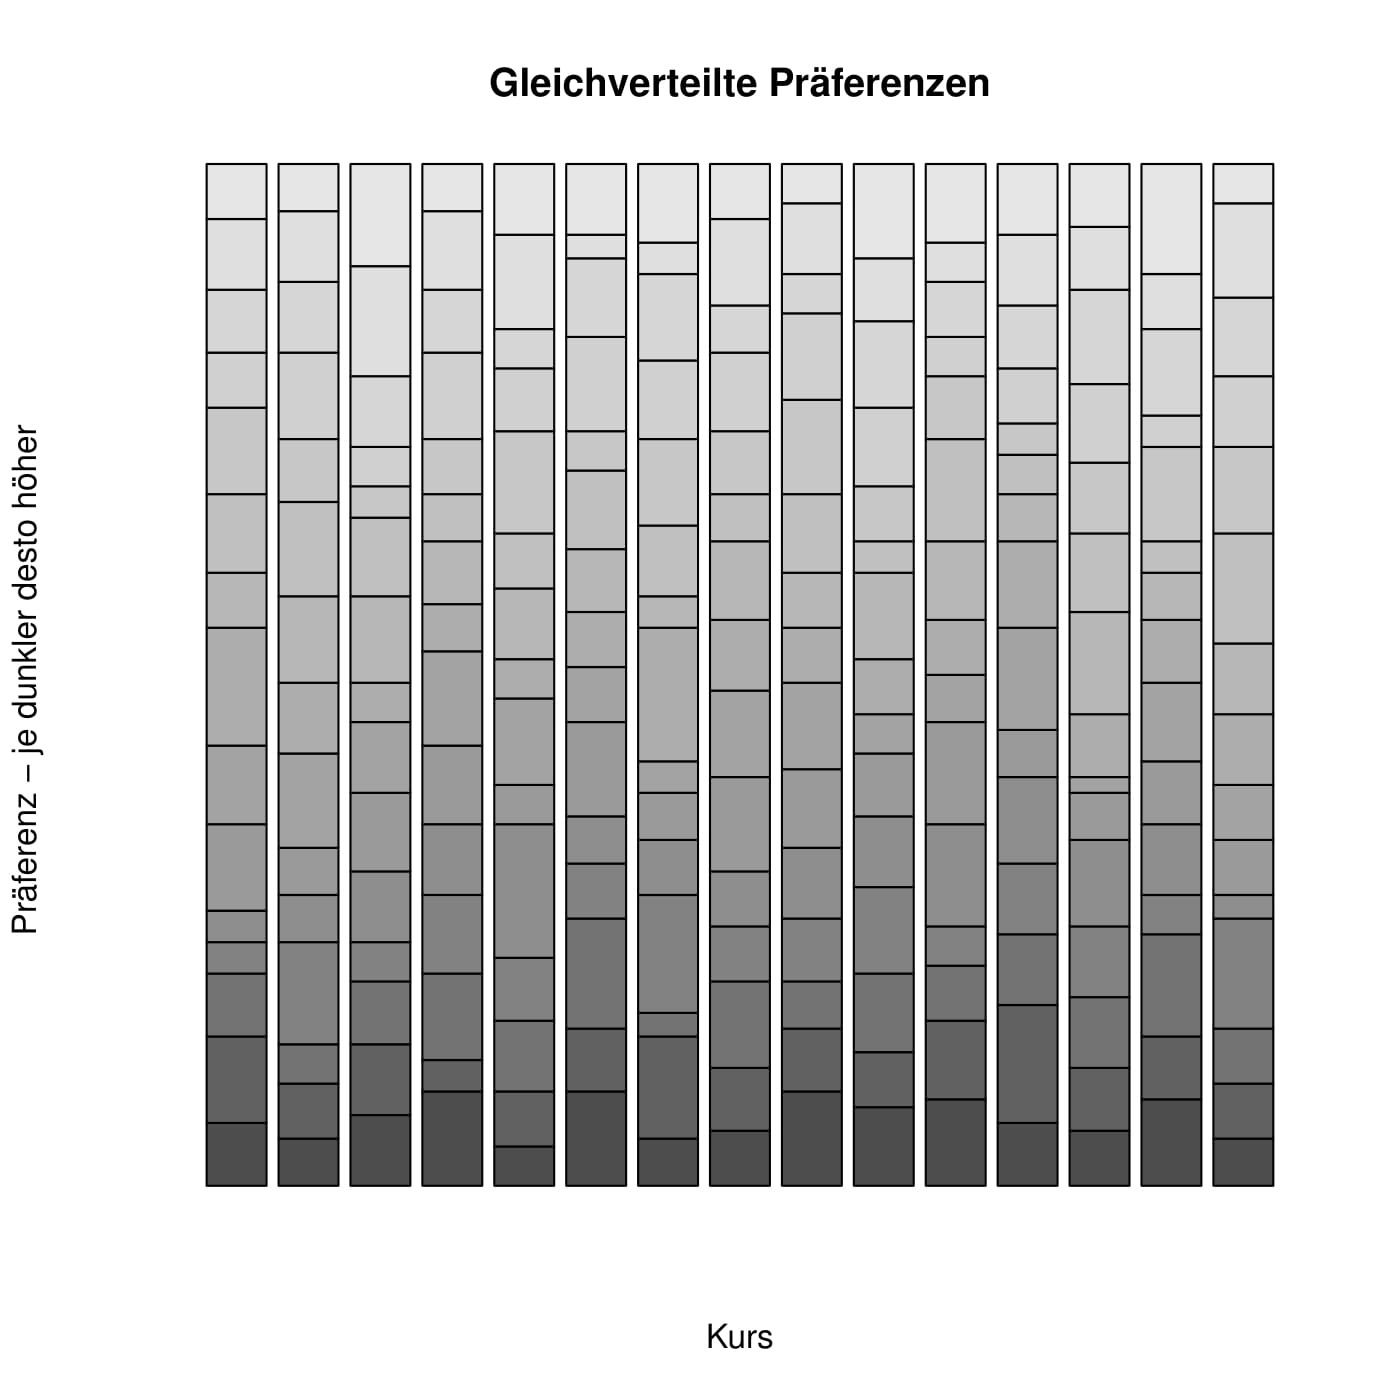
\includegraphics[width=0.7\textwidth]{./testing/images/EqualDistPreferencesDist.jpg}
				\caption{Gleichverteilte Präferenzen mit 130 Studenten auf 15 Kursen mit maximal 10 Teilnehmern pro Kurs. Die Dunkelheit stellt die Höhe der Präferenz dar}
				\label{fig:test_equal_distribution}
			\end{figure}
        
			In Abbildung \ref{fig:test_equal_distribution} sind die gleich verteilten Präferenzen zu sehen.
			Das heißt, die Wahrscheinlichkeit, dass ein beliebiger Student einen beliebigen Kurs mit beliebiger Präferenz wählt, ist immer gleich.
			Dennoch ist eine gewisse Streuung in der Ziehung der Präferenzen zu beobachten.        
			Daher hat jeder Kurs leicht unterschiedlich viele Studenten pro Präferenz.
   	
			\begin{figure}
				\centering
				\begin{subfigure}{0.49\textwidth}
					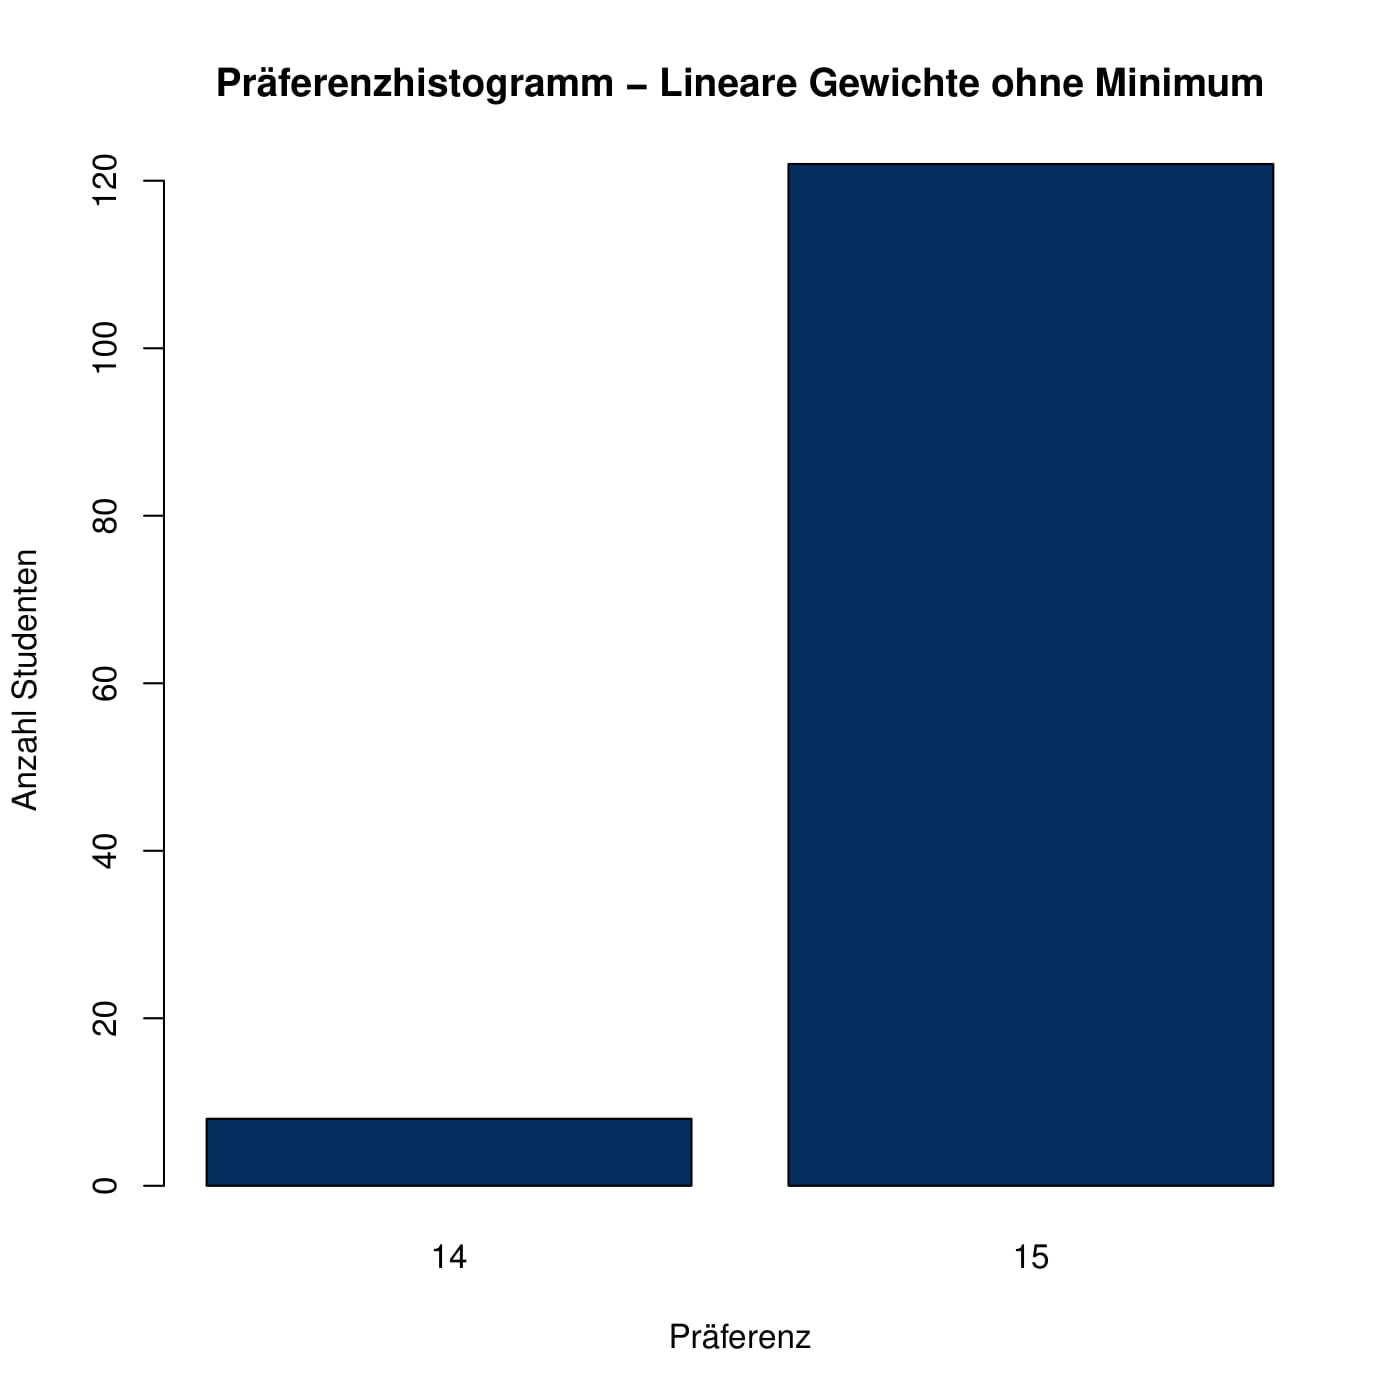
\includegraphics[width=1.0\textwidth]{./testing/images/EqualDistPreferencesHistLin.jpg}
				\end{subfigure}
				\begin{subfigure}{0.49\textwidth}
					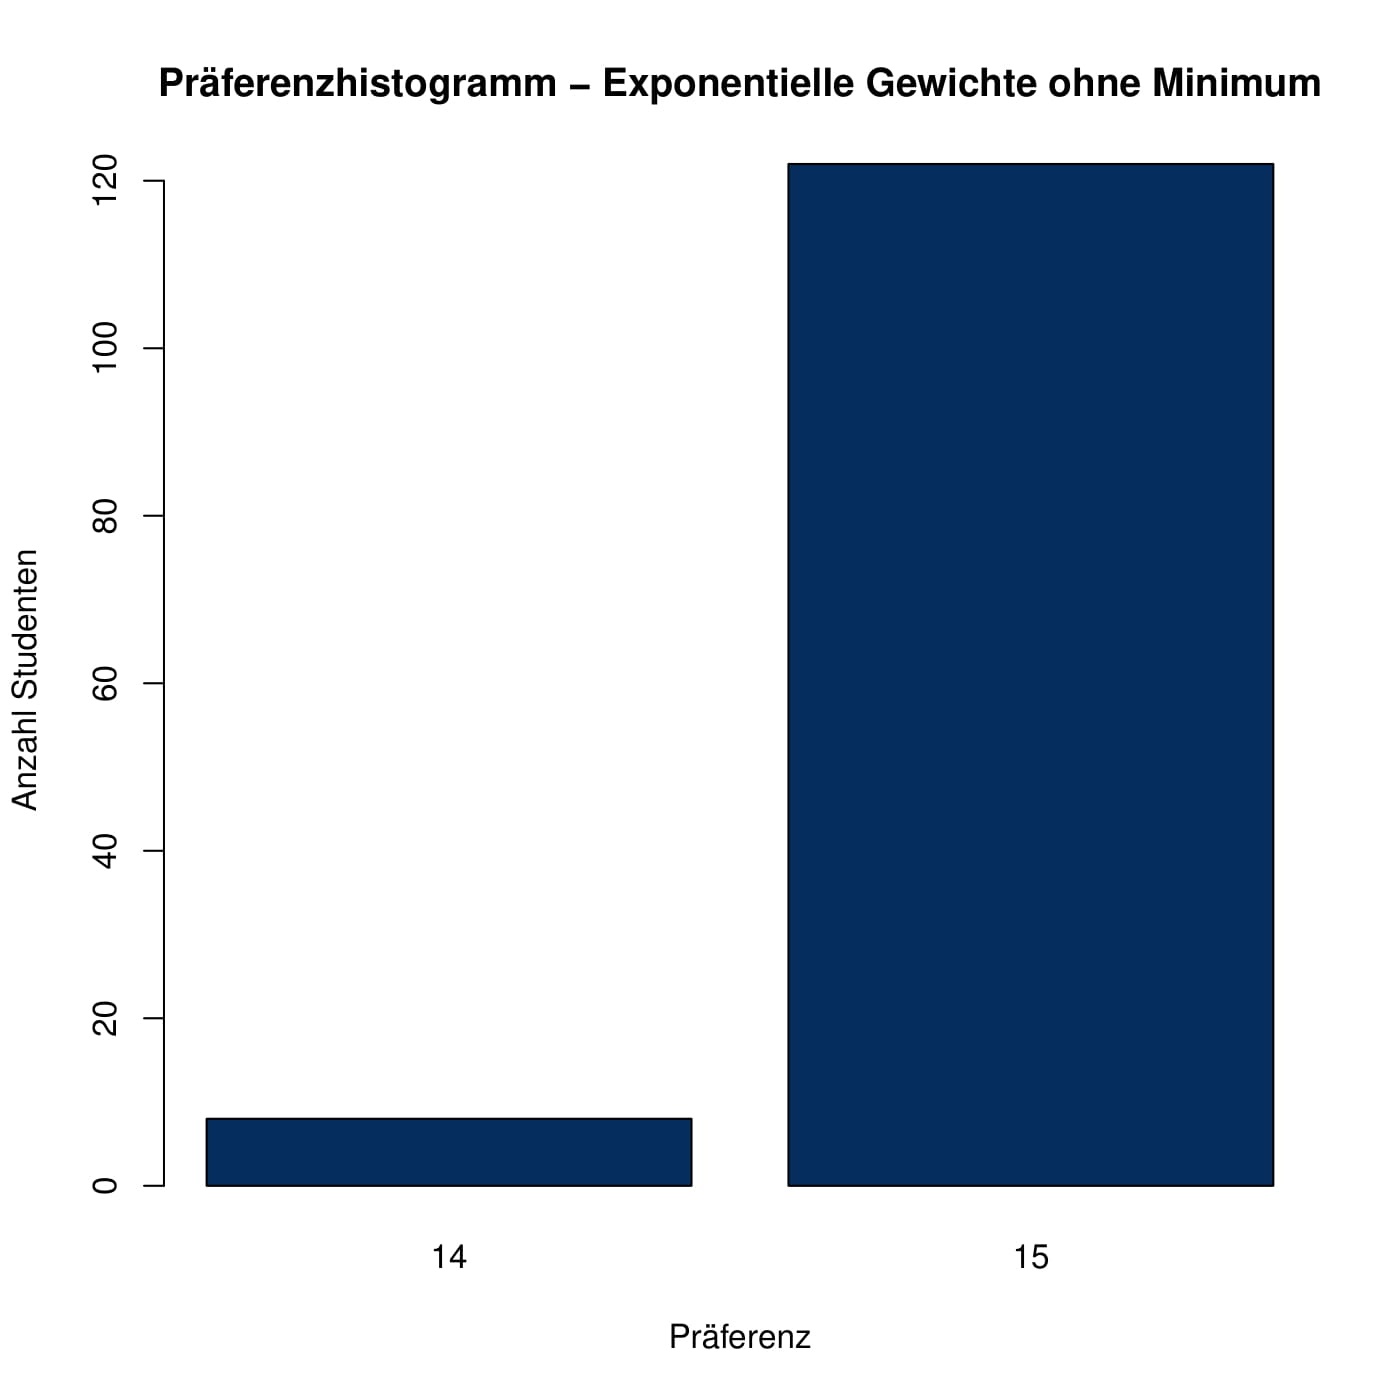
\includegraphics[width=1.0\textwidth]{./testing/images/EqualDistPreferencesHistExpo.jpg}
				\end{subfigure}
				\caption{Gegenüberstellung der Präferenzenhistogramm für lineare und exponentielle Gewichtung}
				\label{fig:test_equal_distribution_histogram}
			\end{figure}
			
			Das Ergebnis des Verteilungsalgorithmus ist in Abbildung \ref{fig:test_equal_distribution_histogram} dargestellt.
			Es ist zu sehen, dass die meisten Studenten ihrer Erstwahl, das heißt dem Kurs mit Präferenz 15, zugeteilt werden.
			Nur sehr wenige Studenten werden in  ihre Zweitwahl verteilt.
			
			Der Grund für diese derart gut Verteilung ist, dass die Präferenzen auf die Kurse gleich verteilt werden.
            Wären die Präferenzlisten exakt gleich verteilt, dann könnte jeder Student dem Kurs mit Präferenz 15 zugeteilt werden.
            Durch die oben erwähnte leichte Streuung, muss es allerdings Studenten geben, die nicht ihrer Erstwahl zugeordnet werden.
            
            Die Variante mit einem festen Minimum wurde nicht getestet, da es nicht möglich ist, ein höheres Minimum zu erreichen.
		
		\subsection{Normalverteilung}
		\label{sec:testing:normaldistribution}
		
			\begin{figure}
				\centering
				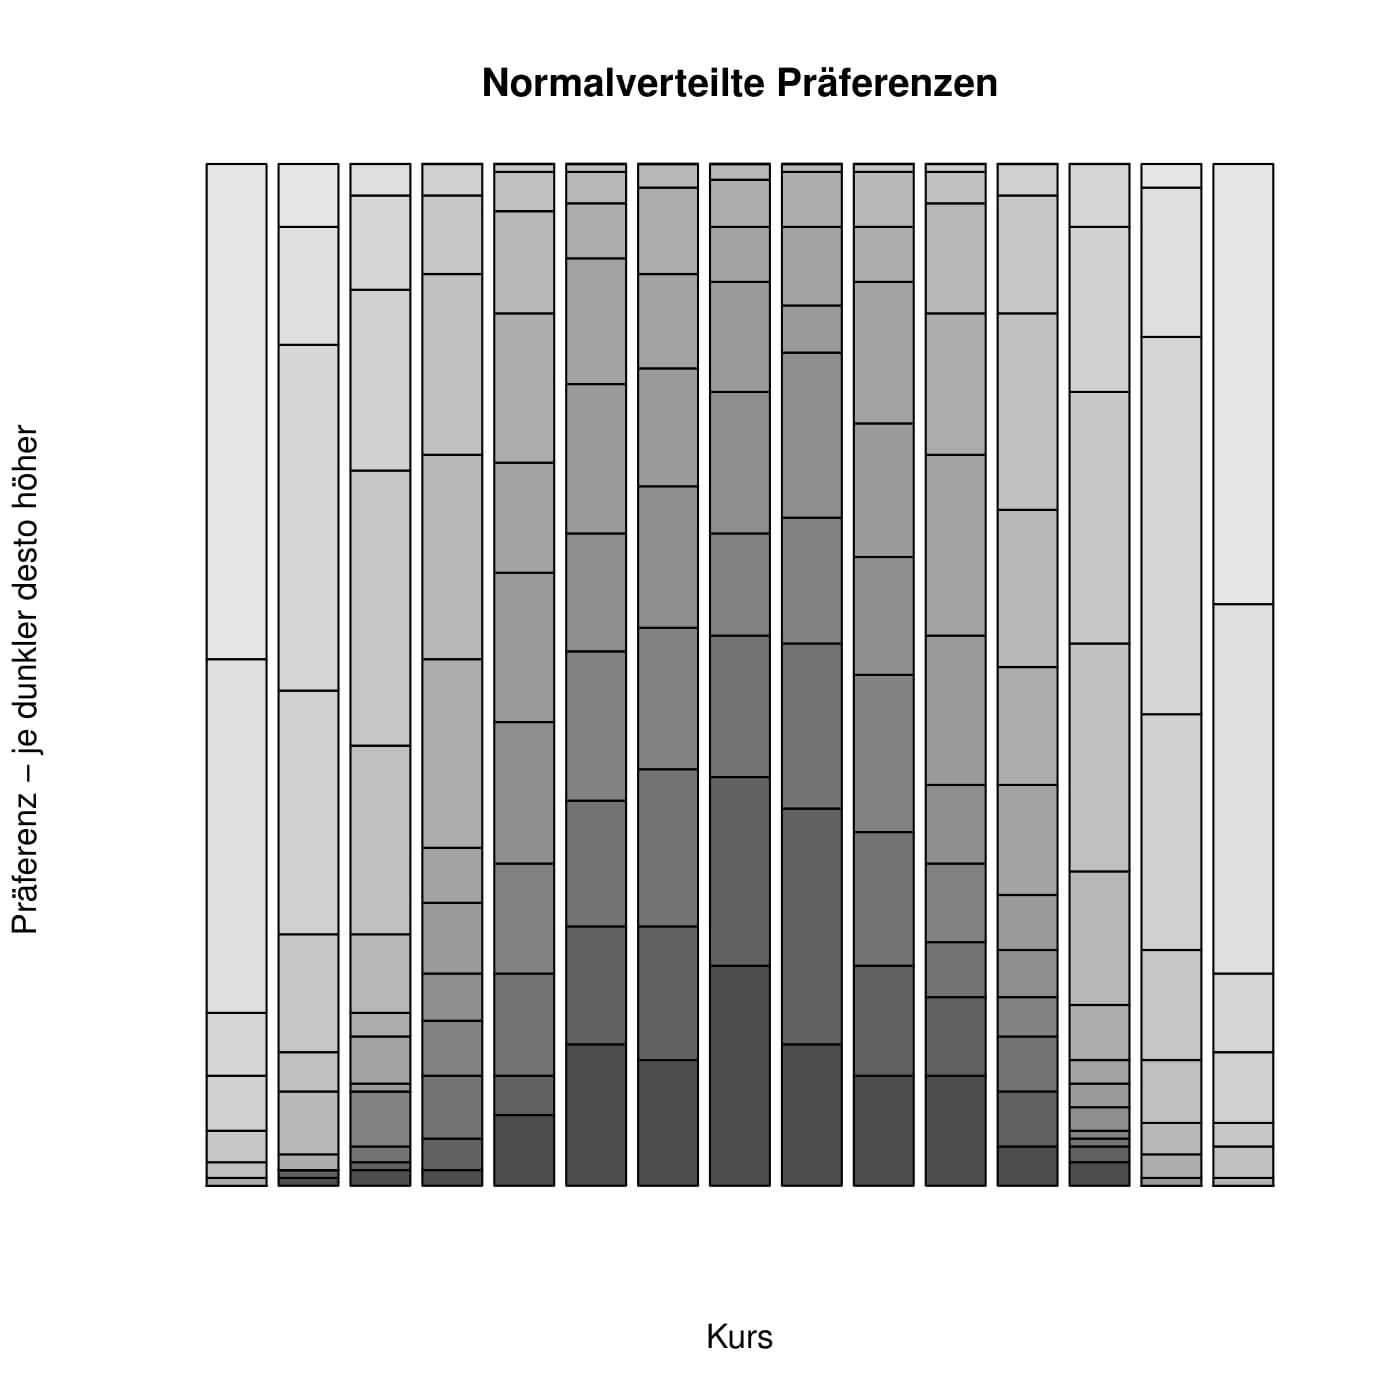
\includegraphics[width=0.7\textwidth]{./testing/images/NormalDistPreferencesDist.jpg}
				\caption{Normalverteilte Präferenzen mit 130 Studenten auf 15 Kursen mit maximal 10 Teilnehmern pro Kurs. Die Dunkelheit stellt die Höhe der Präferenz dar}
				\label{fig:test_norm_distribution}
			\end{figure}
        
			Abbildung \ref{fig:test_norm_distribution} zeigt die normal verteilten Präferenzlisten.
            Es ist zu sehen, dass manche Kurse deutlich häufiger it hohen Präferenzen angegeben wurden.
            Basierend auf diesen Präferenzlisten, ist davon auszugehen, dass nicht alle Studenten ihrer Erst- oder Zweitwahl zugeordnet werden.
			
			\begin{figure}[ht]
				\centering
				\begin{subfigure}{0.49\textwidth}
					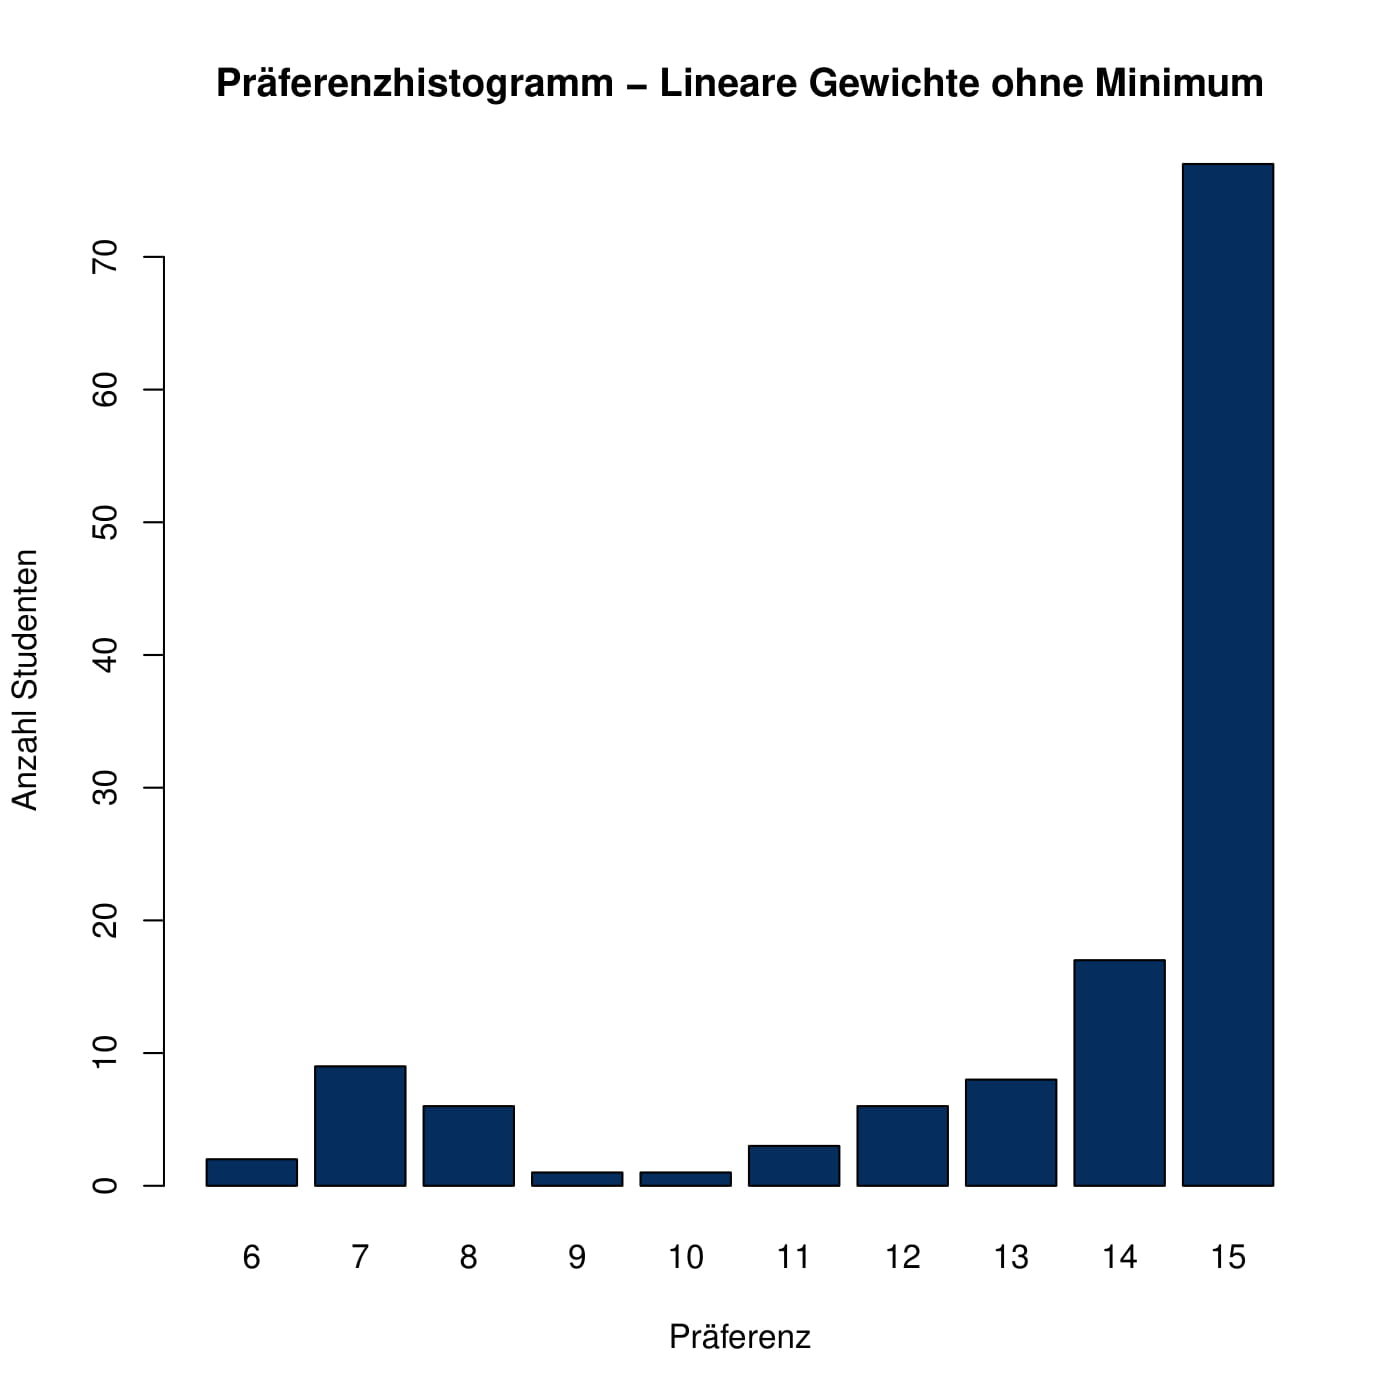
\includegraphics[width=1.0\textwidth]{./testing/images/NormalDistPreferencesHistLin.jpg}
				\end{subfigure}
				\begin{subfigure}{0.49\textwidth}
					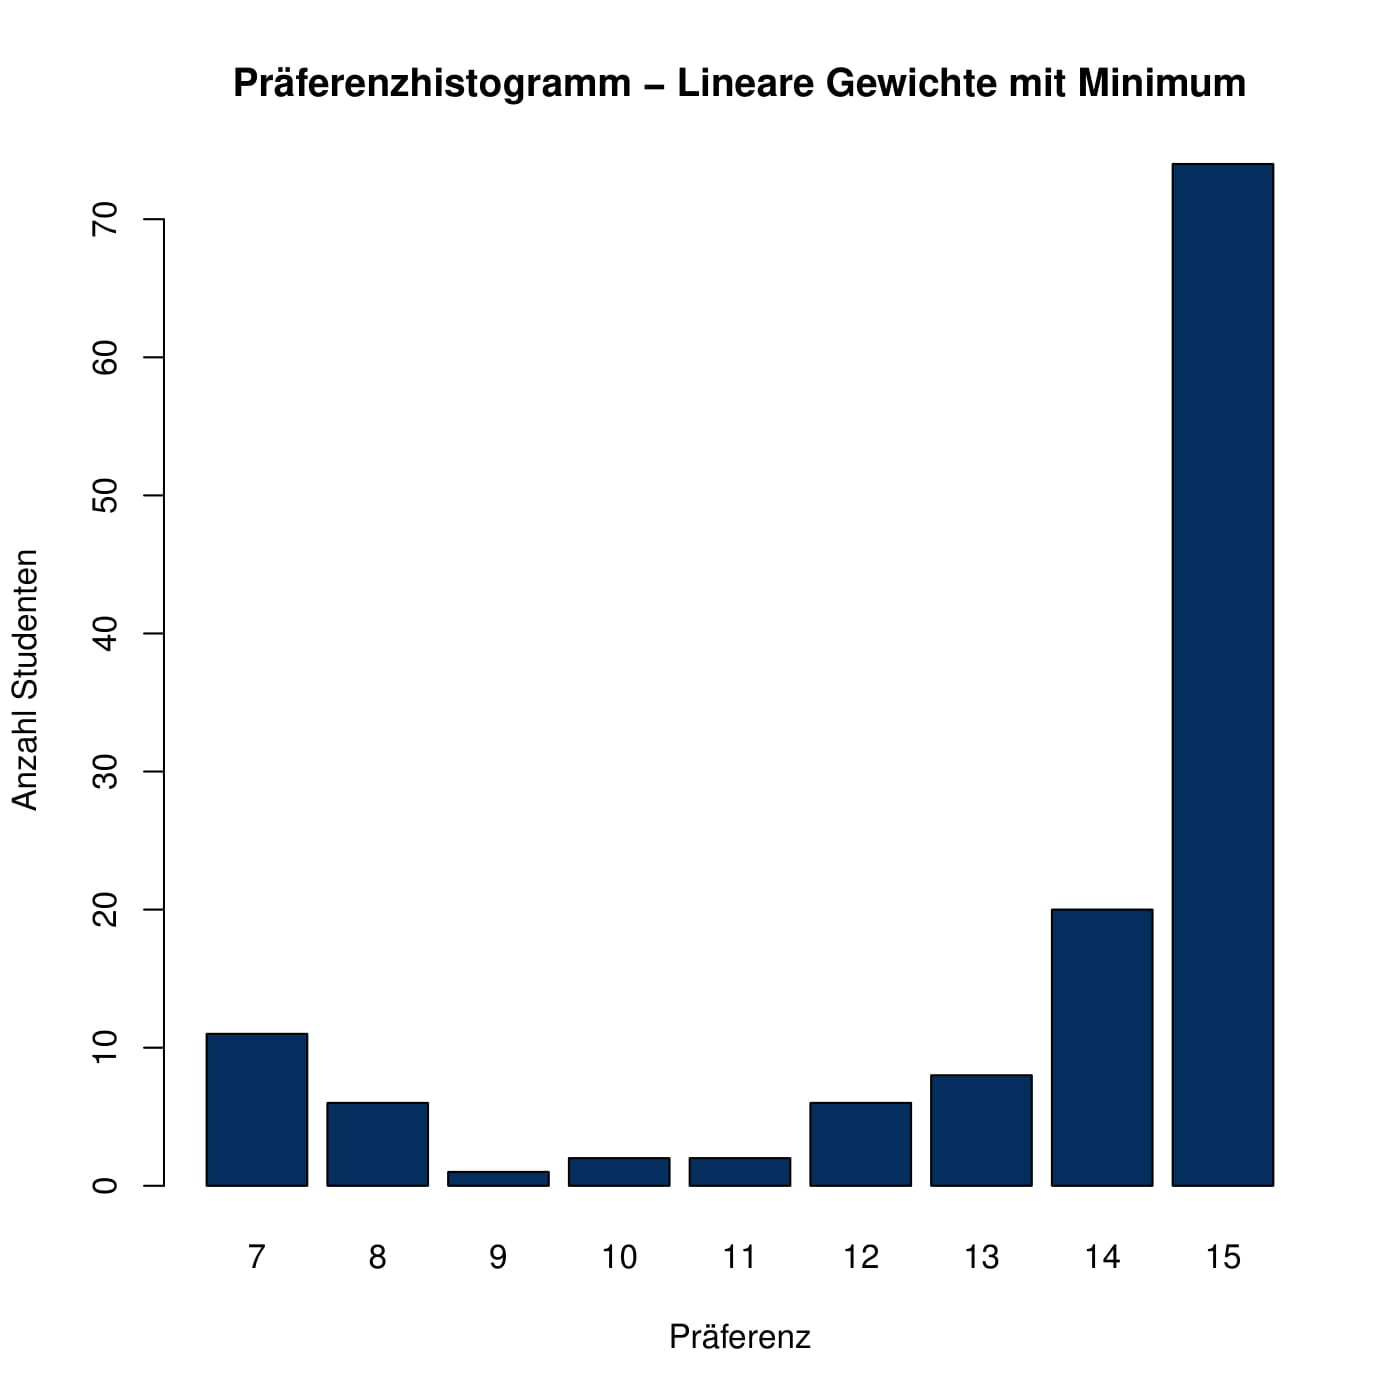
\includegraphics[width=1.0\textwidth]{./testing/images/NormalDistPreferencesHistLinMin.jpg}
				\end{subfigure}
			\begin{subfigure}{0.49\textwidth}
				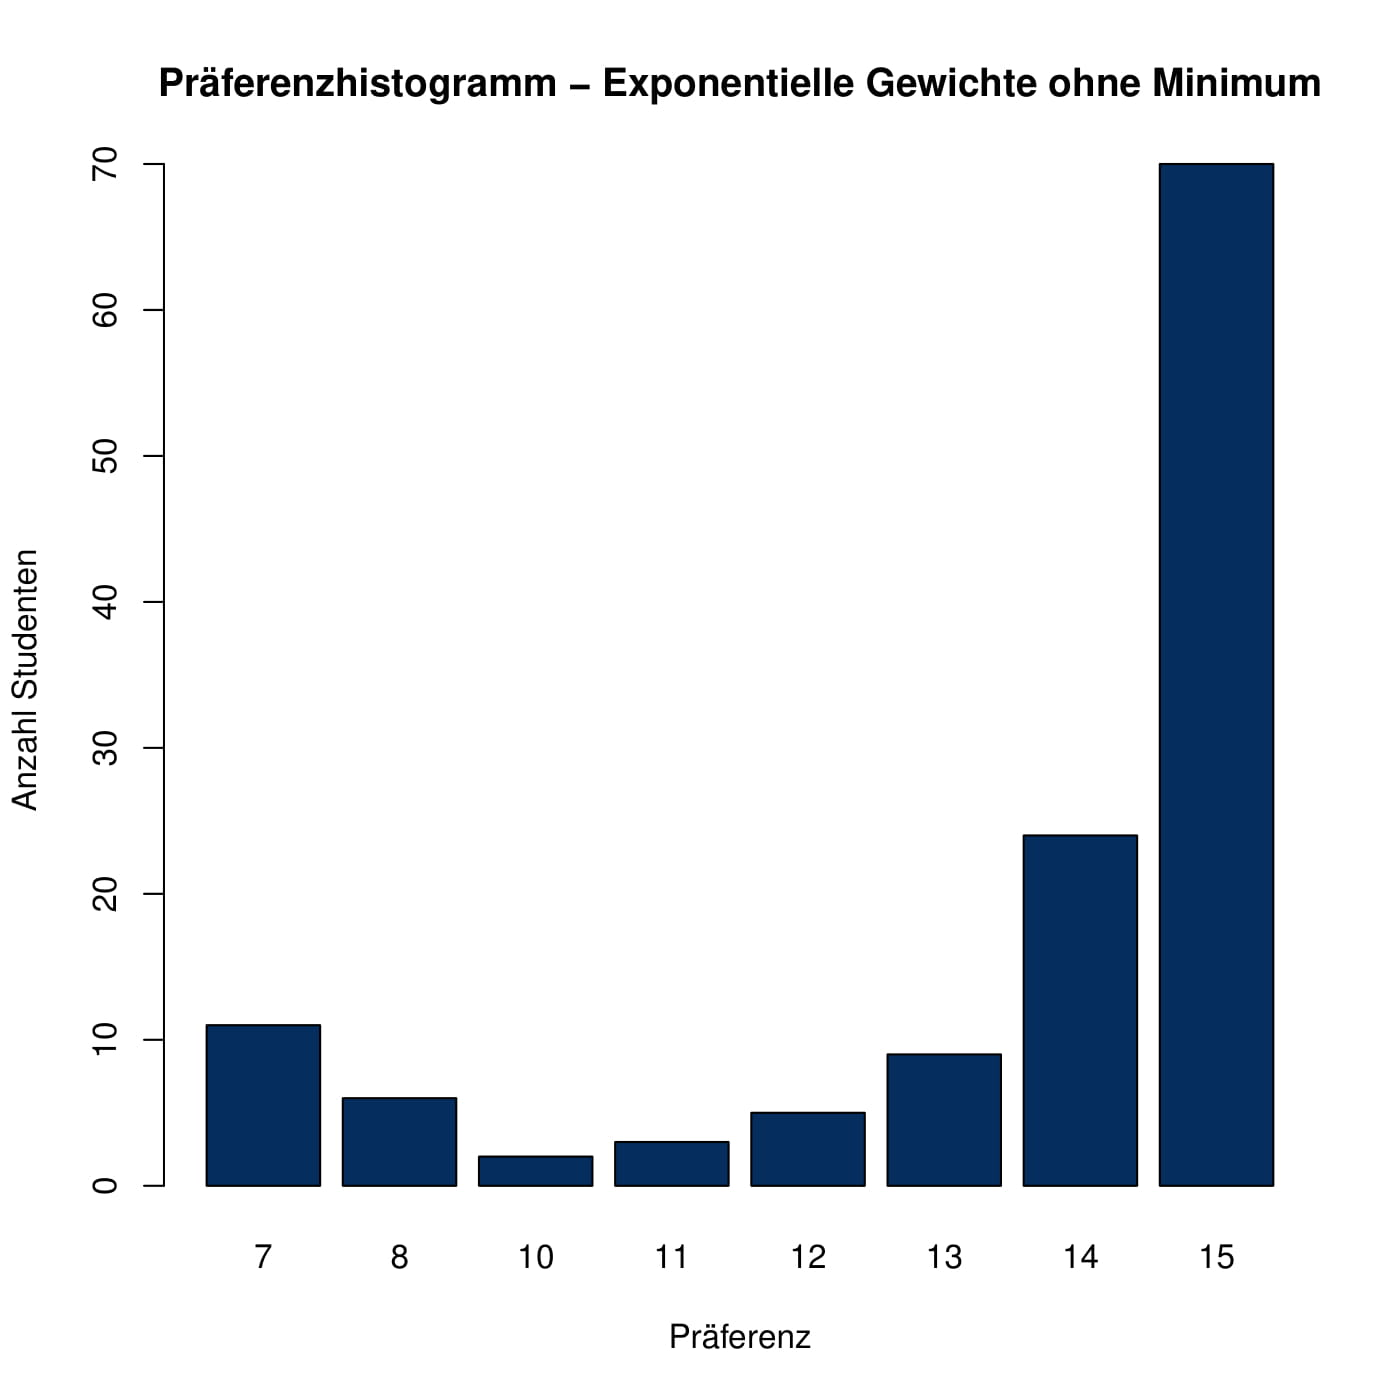
\includegraphics[width=1.0\textwidth]{./testing/images/NormalDistPreferencesHistExpo.jpg}
			\end{subfigure}
				\caption{Gegenüberstellung der Präferenzenhistogramm für lineare Gewichtung, lineare Gewichtung mit Minimum und exponentielle Gewichtung}
				\label{fig:test_norm_distribution_histogram}
			\end{figure}
		
			Das Ergebnis des Verteilungsalgorithmus ist in  Abbildung \ref{fig:test_equal_distribution_histogram} dargestellt.\newline
			
			Wie man sieht, kommen immer noch mehr als die Hälfte der Studenten in ihre Erstwahl.
			Um die 20 Studenten werden allerdings nur einem Kurs mit einer Präferenz kleiner 11 zugeteilt.\newline
			
			Gut zu sehen ist, dass die Variante \glqq Lineare Gewichte ohne Minimum\grqq~sich von \glqq Lineare Gewichte mit Minimum\grqq~unterscheidet.
			Die erste Variante hat die minimale Präferenz 6, doch durch das Erzwingen eines festen Minimums verbessert sich diese auf 7.
			Nach den Anforderungen ist dies so wünschenswert.
			Zuletzt ist in der Variante \glqq Exponentielle Gewichte ohne Minimum\grqq~zu sehen, dass weniger Studenten ihre Erstwahl erhalten, dafür aber mehr Studenten die Präferenz 10 oder höher bekommen.
            Ob dieser Effekt ebenfalls wünschenswert ist, oder aber die Lösung der Variante \glqq Lineare Gewichte mit Minimum\grqq~ vorzuziehen ist, kann hier nicht beantwortet werden. 
			
		\subsection{Realdaten}
		
			Zuletzt wurde der Algorithmus mit realen Daten aus dem Wintersemester 2017/2018 getestet.
            Dadurch ist ein direkter Vergleich mit dem alten Verteilungsalgorithmus möglich.
            Der Datensatz umfasst die Präferenzlisten von 92 Studenten, die auf 15 Kurse verteilt werden sollen.
			
			\begin{table}[h]
				\centering
				\begin{tabular}{l|l|l}
					& Alter Algorithmus & Neuer Algorithmus \\
					\hline
					Mittelwert & 14.2 & 14.4 \\
					Varianz & 1,8 & 0,75 \\
					Minimale Präferenz & 7 & 12 \\
				\end{tabular}
				\caption{Vergleich des alten Algorithmus mit dem neuen Algorithmus}
				\label{tab:old_versus_new_algorithm}
			\end{table}
		
            In Tabelle \ref{tab:old_versus_new_algorithm} sind die Ergebnisse des alten und des neuen Algorithmus gegenübergestellt.
            Für diesen Vergleich wurden lineare Gewichte mit einem festen Minimum von 12 verwendet.
            Es ist zu sehen, dass sich der Mittelwert nur leicht erhöht.
            Die Varianz hingegen sinkt um $ 1.05 $, sinkt also deutlich.
            Die minimale Präferenz steigt im Vergleich zur vorigen Variante des Verteilungsalgorithmus um $ 5 $ an.			
			Daraus lässt sich ableiten, dass der neue Algorithmus zu einem besseren Ergebnis führt.
			
		\subsection{Ergebnisse des Algorithmus}
			
			Wie in Abschnitt \ref{sec:testing:normaldistribution} bereits erläutert, führen die verschiedenen Varianten des Algorithmus zum Teil zu unterschiedlichen Ergebnissen.
			Nach den Anforderungen aus Kapitel \ref{chapter:requirements}, soll der Administrator die Wahl haben, welches Verteilungsergebnis genutzt werden soll.
            Um die korrekte Funktionalität dieser Ergebnisauswahl zu testen, wurden mehrmals Verteilungen generiert und im Anschluss sicher gestellt, dass die entsprechenden Verteilungen ins System übernommen wurden.
            Dies wurde realisiert, indem die minimale Präferenz der eingetragenen Nutzer mit dem theoretischem Ergebnis verglichen wurde.\\

			Gleichzeitig wurde verifiziert, dass ein Bestätigen der Verteilung die entsprechenden E-Mail-Benachrichtigung nach sich zieht.
			Dafür wurde ein Mailserver genutzt, der die E-Mails aller Benutzer erhält.
			Nach den Anforderungen as Kapitel \ref{chapter:requirements} sollten hierbei drei Typen von Mails verschickt werden.
			Studenten erhalten eine E-Mail mit Informationen, welchen Kurs sie zugeteilt wurden.
			Dozenten erhalten eine E-Mail mit Informationen, welche Studenten in ihren Kursen sind.
			Administratoren erhalten eine E-Mail mit Informationen, welche Studenten welchen Kurs bekommen haben.
            
			Für die Verifikation wurde jeweils eine E-Mail der Rolle gewählt und die Richtigkeit der Informationen überprüft.	
